\title{Big Data Analytics in Detection of DDoS (Distributed Denial-of-Service) attacks}


\author{Neha Rawat}
\affiliation{%
	\institution{Indiana University}
	\city{Bloomington} 
	\state{Indiana} 
}
\email{nrawat@iu.edu}



% The default list of authors is too long for headers}
\renewcommand{\shortauthors}{N. Rawat}


\begin{abstract}
	With the increase in internet traffic, threats on the network have also increased. Denial-of-service attacks are cyber attacks wherein a perpetrator, due to any kind of malicious intent, tries to make a resource on the network unavailable to its intended users and carries it out by swamping the system or resource with excess requests in order to overload it and prevent users from accessing it. A much more dangerous variety of such an attack is if it is distributed i.e. coming from various sources. Big Data analytics, however, can be used to detect such attacks by having the ability to store the voluminous logs of such attacks and using the data and machine learning techniques to design an anomaly detection system (using a classification model) to detect and prevent these attacks. This project wil aim to explore such classification models, design and train the most optimum model and display its effects using a DDoS network traffic logs dataset.
\end{abstract}

\keywords{i523, HID224, Denial-of-Service, Intrusion Detection, KDD Cup'99 dataset, Machine Learning, Apache Spark}

\maketitle

\section{Introduction}
The Internet allows us several comforts and functionalities in our day-to-day lives. With the increasing flexibility and accessibility provided by technology, the Internet has become and indispensable part of our life. However, this same accessibility often provides openings for malicious attackers to enter. Security over the Internet is an interdependent factor, with the security of one user depending on rest of the global network (cite1). Denial-of-Service attacks are attacks by such malicious users in order to disrupt the accessibility of other legitimate users to a Web Service or application (cite2). The objectives of such attacks are mainly malicious, driven out of revenge or for some material gain. The attacks seriously hinder the productivity of the victim, as the resources available are not sufficient to handle the oncoming flood of requests. This attack increases in complexity when there are multiple sources of attacks, resulting in a Distributed Denial-of-Service attack. ``In the case of a Distributed Denial-of-Service (DDoS) attack, an attacker uses multiple sources - which may be compromised or controlled by a group of collaborators - to orchestrate an attack against a target'' (cite2). A small batch of requests sent by an attacker may be enough to generate a large amount of unwanted traffic. The earliest of these attacks was when a DDoS tool called Trinoo, deployed in at least 227 systems, flooded a University of Minnesota computer, which was subsequently rendered useless for more than two days (cite1).
\begin{figure}
	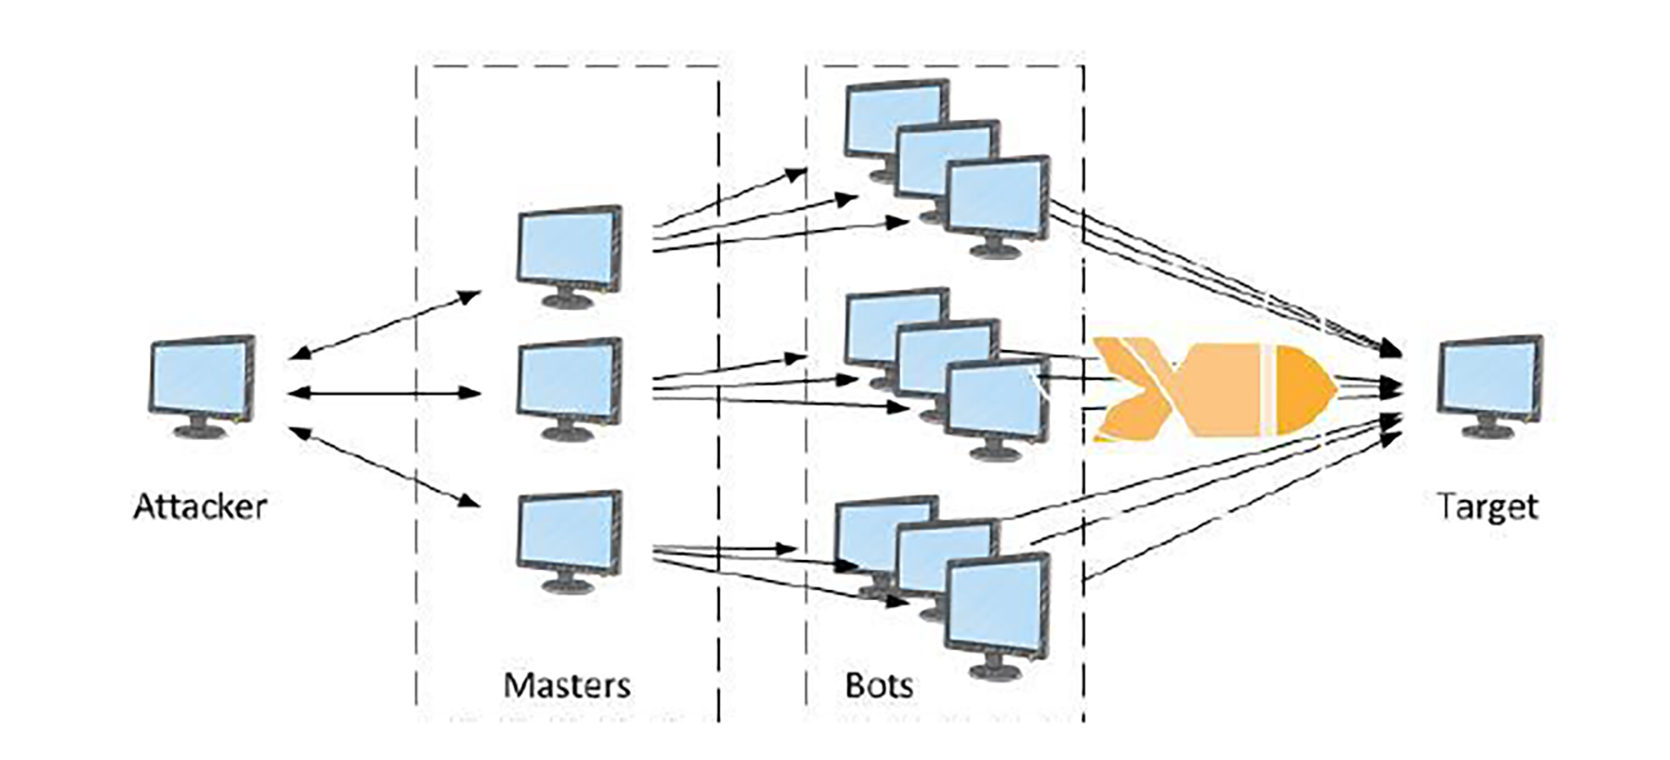
\includegraphics[width=1.0\columnwidth]{images/DDoS.PNG}
	\caption{Distributed Denial-of-Service Attack (cite2)}
	\label{F:ddos}
\end{figure}
Figure \ref{F:ddos} shows how a Distributed Denial-of-Service attack occurs.\\
As the connectivity increases in our everyday lives, so have the risks for DDoS attacks. The Internet of Things (IoT) for example, has opened up a whole new avenue for Denial-of-Service attackers. Earlier, limited to attacks over the Internet which mostly affected a user's computer, with the advent of IoT, the scope of attacks on other smart devices has increased considerably. These devices could be used as pawns in a DDoS attack network and could even be the intended targets for such an attack. Some of the largest DDoS attacks till date are as given: In March of 2013, the DDoS attack on Spamhaus saw 120 Gbps of traffic on their network, in August of 2013, a ``part of the Chinese internet went down in one of the largest DDoS attacks'', in the Spring of 2015, UK-based phone carrier Carphone Warehouse got attacked and hackers stole millions of customers’ data and in January of 2016, some HSBC customers were inhibited from accessing their online banking accounts, which caused a great upheaval as it was ``two days before the tax payment deadline in the United Kingdom'' (cite3). We can see that these attacks, if allowed to happen, have great damage potential. Hence, DDoS mitigation service providers like Imperva Incapsula Enterprise, Arbor Cloud, Verisign, DOSarrest and CloudFlare, have their work cut out for them to detect and prevent such attacks, which are increasing in their reach and complexity (cite4).
   

\section{DDoS Attack Types and Architecture}
In order to prevent a DDoS attack, it is important to know the points in a network where the attack is expected to occur and the type of attack that can occur. Referring to an Open Systems Interconnection(OSI) model, we can usually narrow down the layers which could be affected by a potential attack to the Network, Transport, Presentation and Application layers (cite2).
\begin{figure}
	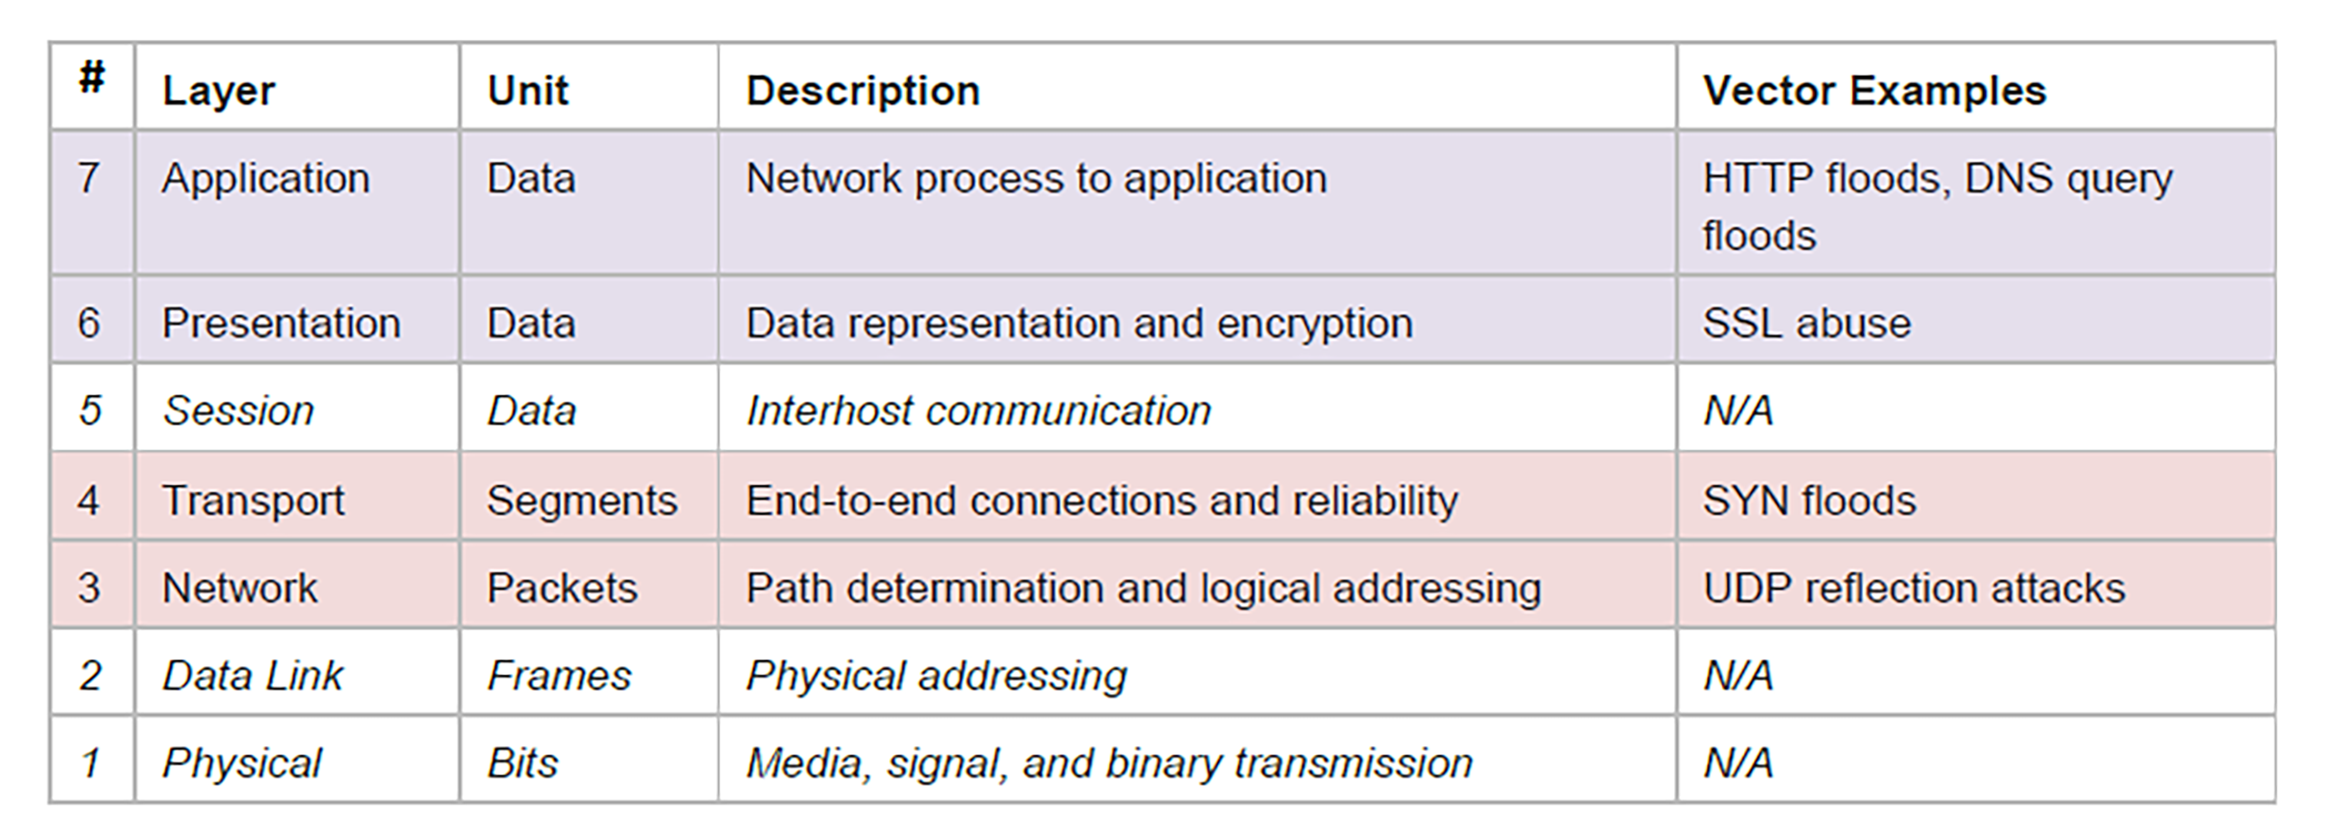
\includegraphics[width=1.0\columnwidth]{images/OSI.PNG}
	\caption{Open Systems Interconnection Model (cite2)}
	\label{F:osi}
\end{figure}
Figure \ref{F:osi} shows an Open Systems Interconnection Model with the layers highlighted where DDoS attacks are most common.\\
Apart from this, the DDoS attacks generally have a specific architecture and follow certain strategies. Knowledge of the pathway which a Denial-of-Service attack follows is essential to detecting and mitigating it.
\subsection{DDoS Attack Types}
The DDoS attacks in the Network and Transport layers are generally of the User Datagram Protocol (UDP) reflection and synchronize (SYN) flood types (cite2). The UDP protocol can allow the attacker to fake the source of a request sent to a server and generate a larger response. The amplification factor of a protocol (request to response size) will result in an overwhelming response to a comparatively smaller request. ``For example, the amplification factor for DNS can be in the 28 to 54 range - which means an attacker can send a request payload of 64 bytes to a DNS server and generate over 3400 bytes of unwanted traffic'' (cite2). A SYN flood attack is based on employing all the resources of a system and exhausting them by leaving connections half-open. For example, when an user connects to a TCP service, the client will send a SYN packet and the server will return a SYN-ACK, expecting the client to return an ACK and completing the handshake. In a SYN flood attack, the ACK is not returned and so the server is stuck in this state which prevents other users from connecting to it (cite2).\\
In the Presentation and Application layers, the DDoS attacks are slightly different. The most common of such attacks are ``HTTP floods, cache-busting attacks, and WordPress XML-RPC floods'' (cite2). In an HTTP flood attack, the attacker sends HTTP requests under the guise of a real user or web service. These attacks target a resource or try to emulate human behavior. Cache-busting attacks are a specialized version of HTTP flood attacks that use ``variations in the query string to circumvent content delivery network (CDN) caching which results in origin fetches, causing additional strain on the origin web server'' (cite2). A WordPress XML-RPC flood (WordPress pingback flood) is used by an attacker to misuse the XML-RPC API function of a website hosted on WordPress software to generate HTTP flood requests. This type of attack has {\em WordPress} present in the HTTP request header and so is clearly recognizable (cite2).
\subsection{DDoS Attack Architecture}
``DDoS attack networks follow two types of architectures: the Agent-Handler architecture and the Internet Relay Chat (IRC)-based architecture'' (cite1). The components of an Agent-Handler architecture are clients, handlers, and agents. In this type of architecture, the attacker connects with the rest of the attack system at the client point. The handlers are generally software packages available over the Internet which are used by the client to connect to the agents. The agent softwares are placed in the vulnerable systems that are finally used to implement the attack. Often, the users of the agent systems are not aware of the attack being carried out (cite1). In the IRC-based architecture, ``an IRC communication channel is used to connect the client(s) to the agents'' (cite1). IRC ports are employed to send commands to the agents, making the DDoS command packets harder to trace (as these channels have a lot of traffic) (cite1).\\
When launching a DDoS attack, the attacker goes through some steps common to both types of architectures (cite1). First, the attacker tries to identify vulnerable systems that can be used as agents. The resources of these systems are used to generate a powerful attack stream. Next, the attacker plants the handler software code in the compromised system and ensures steps to prevent the code from being detected. These compromised systems are often referred to as {\em zombies}. Sometimes, the attacker creates several intermediate layers between the {\em zombies} and the victim to hinder traceability. Thirdly, the attacker communicates with the handler codes placed via protocols like TCP or UDP, and decides the scheduling of the attacks. Post the complete setup, the attacker launches the attack on the victim's machine or server and renders it unusable (cite1). In an IRC-based architecture, most of the above steps remain same, but an IRC-channel is used for communication purposes. This helps the attacker as even if one {\em zombie} or {\em bot} is discovered, the identities of the others is still hidden, as IRC-channels are difficult to detect (cite1).
\begin{figure}
	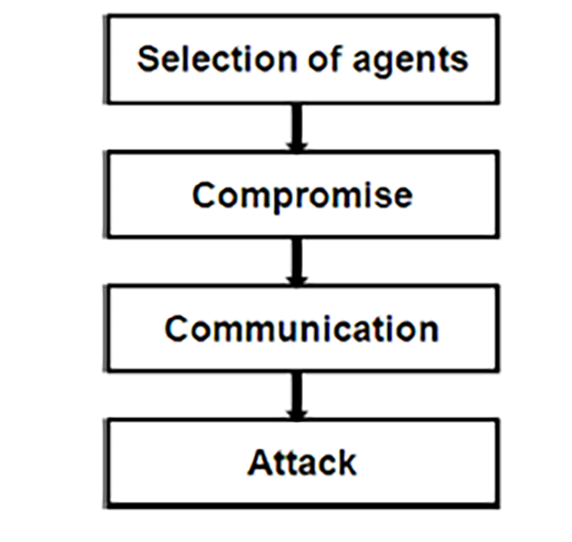
\includegraphics[width=1.0\columnwidth]{images/dossteps.PNG}
	\caption{Steps of a Denial-of-Service attack (cite1)}
	\label{F:doss}
\end{figure}
Figure \ref{F:doss} shows the steps of a Denial-of-Service attack execution.\\

\section{DDoS Attack Defense Methodologies}
In the previous section, we explored the common types of DDoS attacks and the general architecture that they follow. These different types of attacks are used with variation by attackers in their attempts to obstruct utilization of resources.  
\begin{figure}
	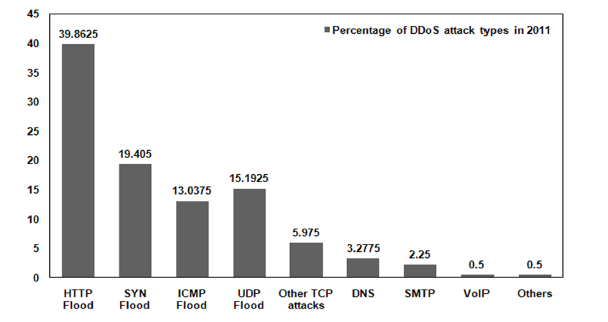
\includegraphics[width=1.0\columnwidth]{images/dosattackstat.PNG}
	\caption{Different Denial-of-Service attack type statistics (cite1)}
	\label{F:dosstat}
\end{figure}
Figure \ref{F:dosstat} shows the percentage of different Denial-of-Service attacks in 2011 by type.\\
The different types of DDoS attacks and their improvement throughout time has also invoked different defense mechanisms against these attacks. DDoS defense mechanisms are usually employed at three points in the attack network : Victim-end, Source-end and Intermediate-Network (cite1). Victim-end detection approaches are generally incorporated in the routers of victim networks. A detection system is used to detect intrusion based on different techniques.  Detecting DDoS attacks at this point is relatively easy and the most practically applicable, but has the disadvantage of detection only after the attack has reached the victim and legitimate users have already been denied services (cite1). Source-end detection system works similarly to the victim-end detection system apart from ``a throttling component'', which is added to force a rate limit on outgoing connections. The detection system then compares both incoming and outgoing network traffic with normal traffic benchmarks to detect an attack. This is probably the ideal defense mechanism, but faces challenges in the deployment of a detection system at the source and difficulty in identification in case of multiple sources (cite1). The intermediate-network defense mechanism acts like a middle-ground between the victim-end and source-end systems. It acts like a collaborative model which depends upon communication and sharing of information between all routers on the network. Hence, this too suffers from the problem of deployability, as even one router missing on the network could hinder the traceback process (cite1).\\
From the above defense mechanism schemes, we can garner that detection of these attacks forms a major part of the preventive process. The most commonly used detection methodologies for defense against DDoS are as follows: Statistical Methods, Soft-Computing and Machine Learning Methods anad Knowledge-Based Methods (cite1).

\subsection{Statistical Methods}
Statistical Methods follow the statistical properties of the distribution of incoming and outgoing network traffic for detection of DDoS attacks. The distributions (or statistical estimates generated using it) are compared with those for a normal traffic signature. An example of the same is the use of cumulative deviation from normal to detect DDoS attacks. Similarly, a periodic deviation analysis from the normal pattern can be used to detect intrusions (cite1). Another example, is the use of a two-sample t-test to detect DDoS signatures by comparing the SYN arrival rate distribution with the distribution of a normal SYN arrival rate (after confirming a gaussian distribution for it). If the difference is considered significant according to the t-test, the traffic is marked as potentially containing attack packets (cite1). A prediction method designed by Zhang et al. (cite5) uses an Auto Regressive Integrated Auto Regressive (ARIMA) model for their detection system.

\subsection{Soft-Computing and Machine Learning Methods}
The voluminous network traffic data generated can be leveraged by a soft-computing system like a neural network or a data mining/machine learning model to design a classifier that differentiates between normal traffic and intrusions. An example is the use of statistical preprocessing for extraction of relevant features from the traffic followed by an unsupervised neural net to classify traffic signatures as either a DDoS attack or normal (cite1). Another case is the use of a Radial Basis Function (RBF) neural network to analyze attack packets and classify them as normal or harmful (cite1). Machine learning algorithms like K-Nearest Neighbors and Support Vector Machines can be used as excellent classifiers for incoming network traffic. Fuzzy networks can also be used in the decision-making process while separating normal traffic packets from potentially harmful ones (cite1).

\subsection{Knowledge-Based Methods}
In knowledge-based methods, network traffic features are compared with predefined patterns of attack. Some examples of knowledge-based
methodologies include ``expert systems, signature analysis, self organizing maps, and state transition analysis'' (cite1). Heuristics can be used to analyze traffic characteristics and classify them as DDoS or otherwise. An excellent example is that of a DDoS detection system which used a ``gossip based communication mechanism'' to exchange information about network attacks
among independent detection nodes in order to use the aggregate data to identify network attacks (cite1). Another model, used temporal-correlation based method to extract features and spatial-correlation for detection to correctly identify DDoS attacks (cite1).

\section{DDoS Attack Detection Model}
For this project, we have worked on the design and implementation of an optimal DDoS detection model (based on Soft-Computing and Machine Learning algorithms) by training and implementing several potential models and creating an ensemble model from the best ones. We have also explored the traffic logs dataset to identify patterns via unsupervised means.

\subsection{Data Description}
The KDD Cup'99 dataset (cite6) has been used for our data analysis. This dataset has been derived from the 1998 DARPA Intrusion Detection Evaluation Program dataset (cite7) which was prepared and managed by MIT Lincoln Labs. The data was simulated to evaluate study in intrusion detection. It comprises of a ``wide variety of intrusions simulated in a military network environment'' (cite6). The original data comprised of around five million records. Hence, we use a 10 percent subset of the original train and test datasets for our analysis purposes.

\subsection{Data Exploration and Processing}
The data exploration and analysis for this project has been implemented using Python on {\em Jupyter Notebook}. The {\em Jupyter Notebook} provides us with ``an open-source web application that allows us to create and share documents that contain live code, equations, visualizations and narrative text'' (cite8).\\
For data loading, we use the {\em Pandas} library in python, which is one of the largest and most flexible data managing libraries and offers a wide variety of options for data handling and manipulation using data frames. After loading the datasets, we explore some of the features of the dataset. From the documentation on the KDD Cup'99 dataset, we know that the data consists of a wide variety of network attacks, but the five main classes of network traffic are as follows: normal (normal network traffic), DoS/DDoS (Denial-of-Service network traffic), R2L (unauthorized access from a remote machine traffic), U2R (unauthorized access to local superuser privileges traffic) and probing. Also, the test dataset consists of an additional 14 attack types which are not present in the training data. However, these new attack types are also a part of the above five categories and the purpose behind their addition in the dataset was to prove that new variants can also be detected using signatures of the preexisting types of attacks.\\
For plotting and visualization purposes, we use {\em Matplotlib} and {\em Seaborn} - two excellent visualization libraries offered by Python. First, we check for nulls in the train and test dataset, but find none. Secondly, we check the three categorical columns in the data, to ensure same levels in both the training and test dataset. We find that the training dataset has an additional level in the {\em service} column. For simplicity, we remove the categorical columns from our analysis dataset and continue our work on only the numerical columns.\\
We now explore the target label column which specifies the {\em attack type} or the network traffic class. We map the labels to five core categories discussed previously and compare them for the training and testing set.
\begin{figure}
	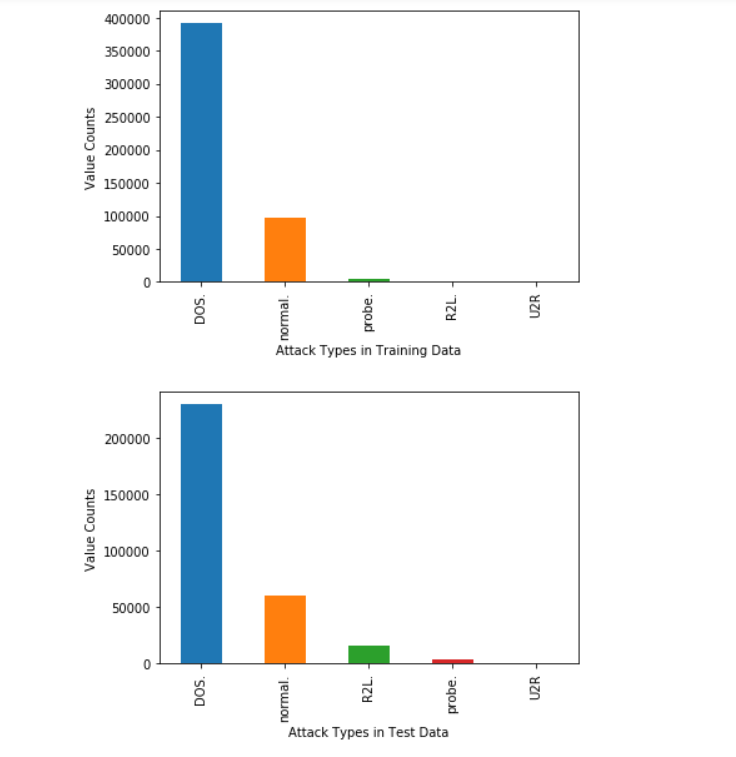
\includegraphics[width=1.0\columnwidth]{images/attack_type.PNG}
	\caption{Attack Type Distributions}
	\label{F:att}
\end{figure}
Figure \ref{F:att} shows the Attack Type distribution in the training and test datasets\\
We can observe that DoS attacks form the majority of all the attack types (98.67 percent out of all attacks in training set; 91.78 percent out of all attacks in test set). Hence, we broadly classify the target labels as {\em normal} and {\em bad} for intrusion detection. We also include the individual labels for the multi-label classification part.\\
Post this, we create pair plots for the first few variables in order to view individual distributions as well as correlations.
\begin{figure}
	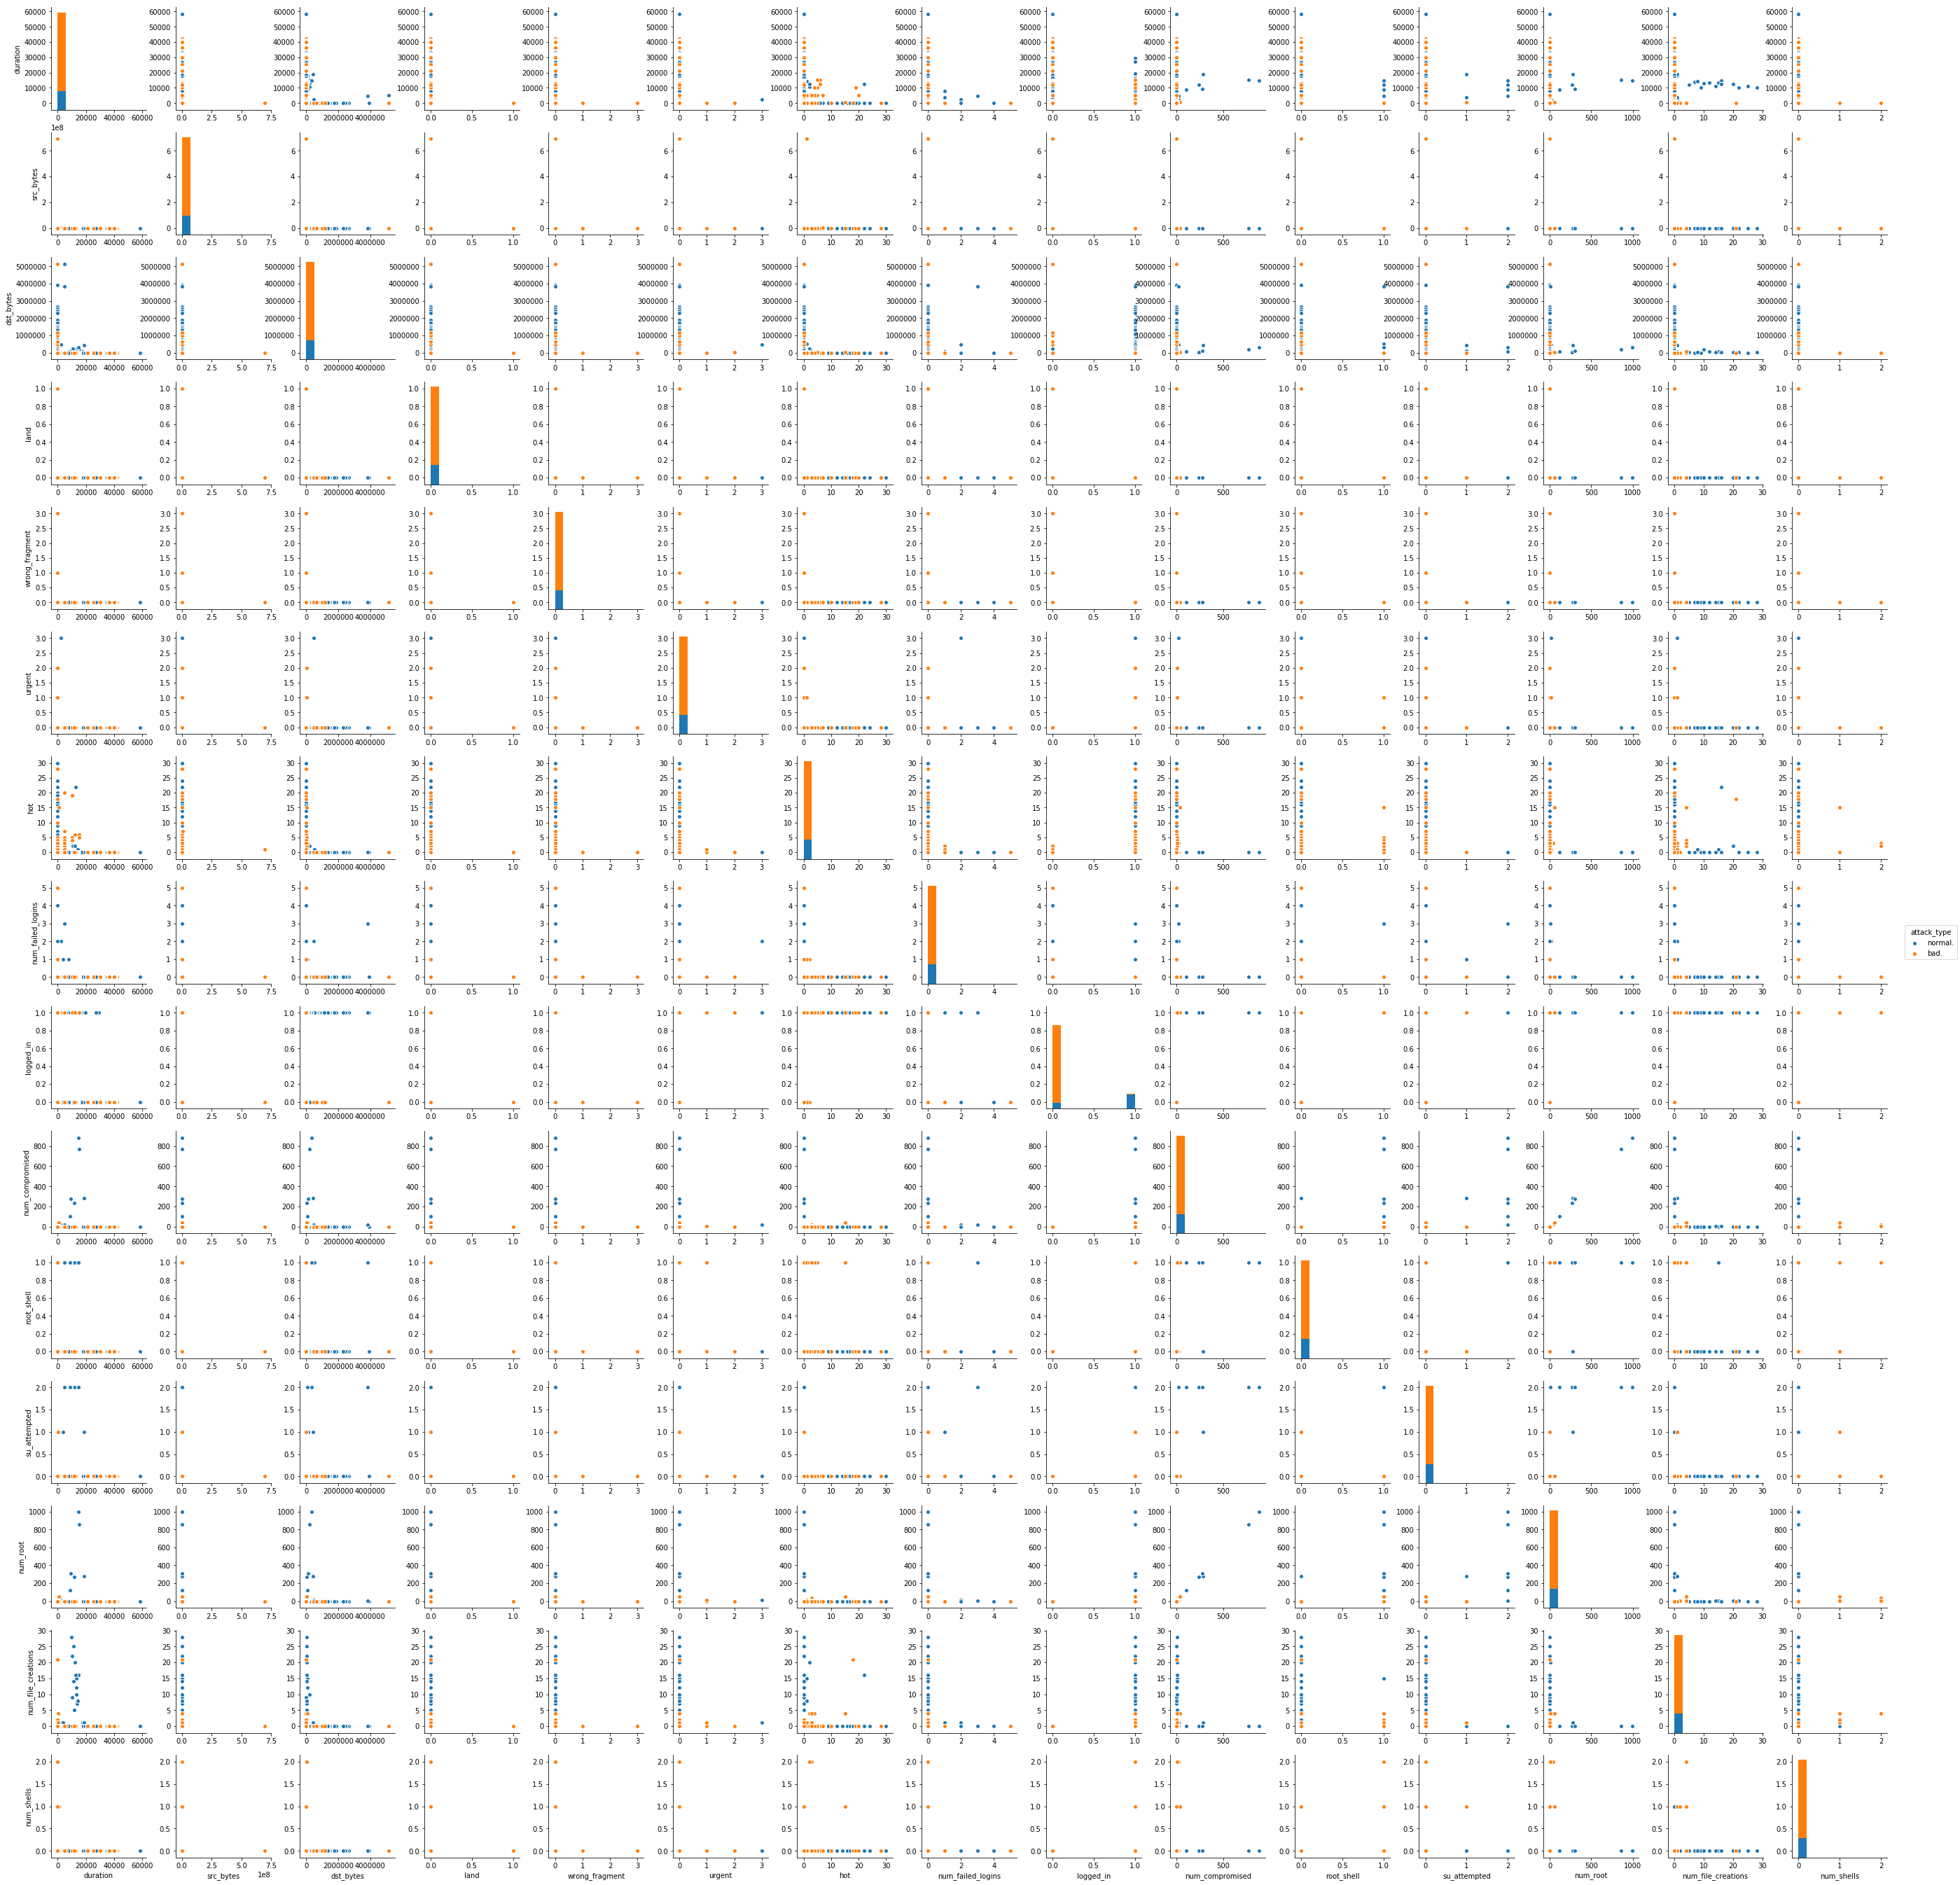
\includegraphics[width=1.0\columnwidth]{images/pairplot.PNG}
	\caption{Pair plot for Training Features}
	\label{F:pair}
\end{figure}
Figure \ref{F:pair} shows the pair plot between the first 15 variables in the training dataset. We observe that the data seems to be skewed, indicating the need for standardizing the features. Also, there do not seem to be a lot of correlated variables in the dataset.\\
We proceed with separating the binary variables (mentioned in the documentation) from the continuous variables and scaling the continuous variables using mean normalization in the training dataset. We then apply the same transformations to the test dataset. Post this, we consolidate all our features and get the final processed datasets for training and testing.

\subsection{Data Analysis}
Once we are ready with our final datasets, we design the required detection models by training them on the training data and testing their performance on the test data. For the design of the models, we use the {\em scikit-learn or sklearn} package in python, which contains a plethora of resources for statistical and machine learning methodologies. For performance tests, we calculate the accuracy, precision, recall and F1 score for the model (for both 2-label and multi-label classification). The confusion matrix generated in each case displays the classes as follows: 2-class classification (0 - bad, 1 - normal) ; Multi-class classification (0 - DoS/DDoS, 1 - R2L, 2 - U2R, 3 - normal, 4 - probe).

\subsubsection{Logistic Regression}
Logistic Regression is a machine learning algorithm based on the regression model which is used to fit a model to describe the relationship between a dependent (categorical target) and one or more independent variables. Used mainly for classification purposes, the target variable in a logistic regression model is mainly binary, although the method can be used for multi-class classification too. The basis of logistic regression is a {\em logistic function} (usually a sigmoid function) which keeps the output values bounded between 0 and 1 (cite9).\\
We train two logistic regression models - one for the 2-class classification and one for the multi-class classification. 
\begin{figure}
	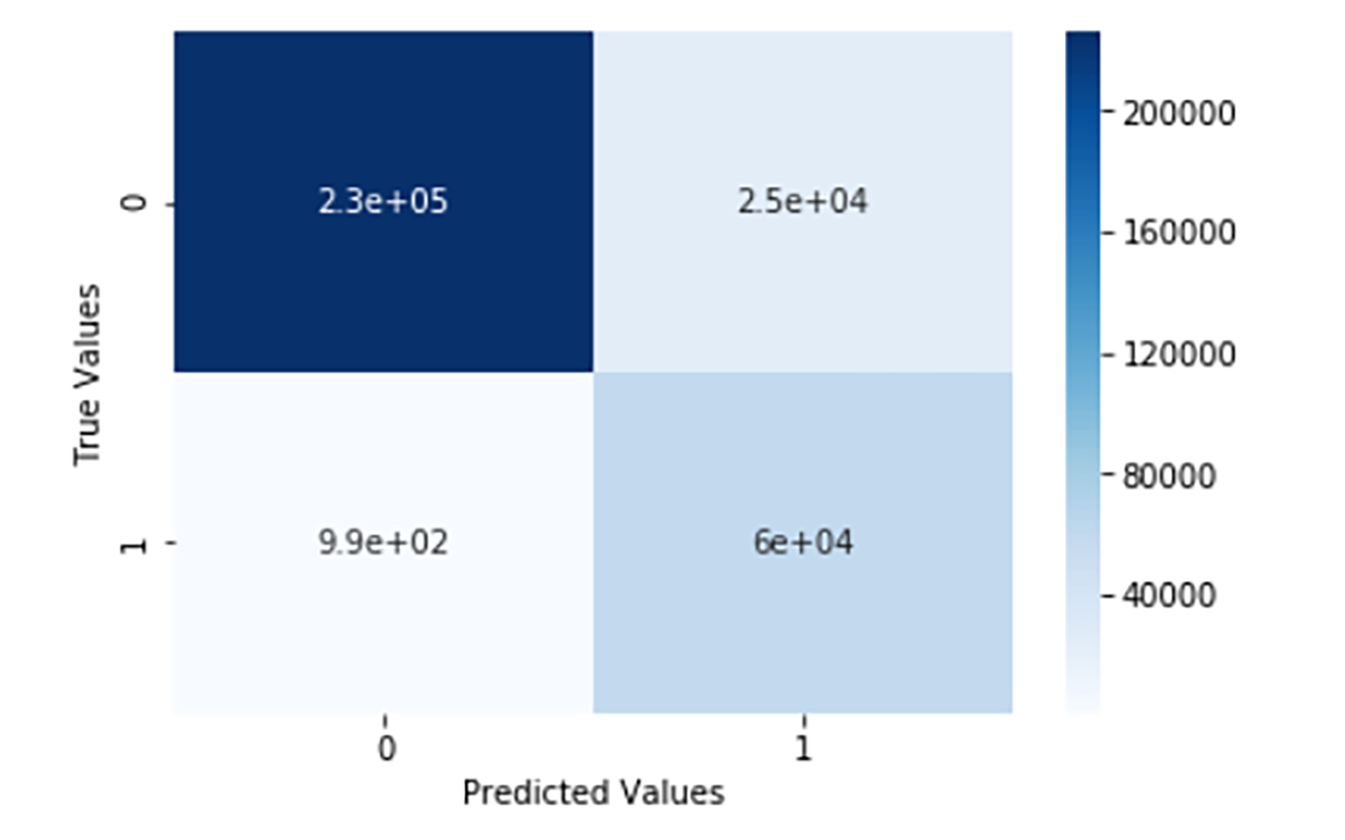
\includegraphics[width=1.0\columnwidth]{images/logreg2.PNG}
	\caption{Logistic Regression Confusion Matrix - 2-class classification}
	\label{F:logreg2}
\end{figure}
Figure \ref{F:logreg2} shows the 2-class confusion matrix for logistic regression.
\begin{figure}
	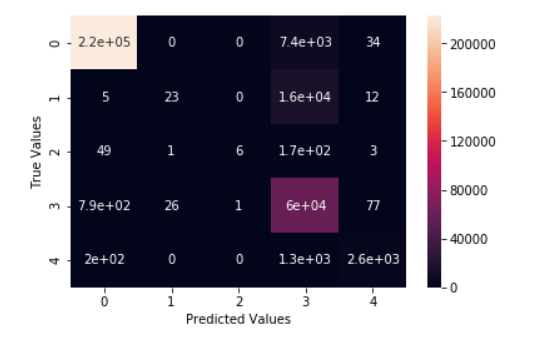
\includegraphics[width=1.0\columnwidth]{images/logregall.PNG}
	\caption{Logistic Regression Confusion Matrix - Multi-class classification}
	\label{F:logregall}
\end{figure}
Figure \ref{F:logregall} shows the multi-class confusion matrix for logistic regression.\\
The overall accuracy, recall, precision and F1 score for the 2-class classification are as follows: 91.7, 94.2, 85.0 and 88.3 percent. The same for the multi-class classification are as follows: 91.5, 52.2, 79.4 and
52.3. We can observe that the accuracy of the model seems to be good for the 2-class classification but the recall and F1 scores decrease for the multi-class classification (due to the decrease in recall for the U2R and R2L classes, which have a higher proportion in test as compared to train data).

\subsubsection{K-Nearest Neighbors}
The K-Nearest Neighbors algorithm selects the {\em k} nearest points to the test data point, present in the training data point, and assign it the class label depending on the majority class label present among the {\em k} training data points(cite9).\\
We train two KNN (k=5) models - one for the 2-class classification and one for the multi-class classification. 
\begin{figure}
	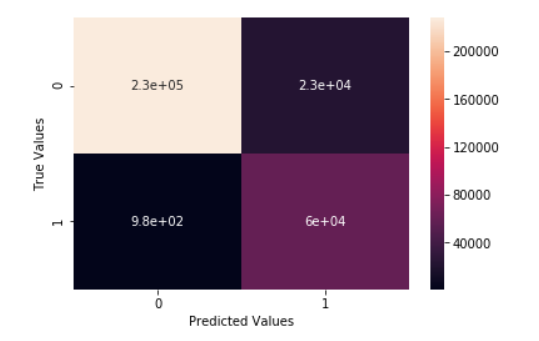
\includegraphics[width=1.0\columnwidth]{images/knn2.PNG}
	\caption{KNN Confusion Matrix - 2-class classification}
	\label{F:knn2}
\end{figure}
Figure \ref{F:knn2} shows the 2-class confusion matrix for KNN.
\begin{figure}
	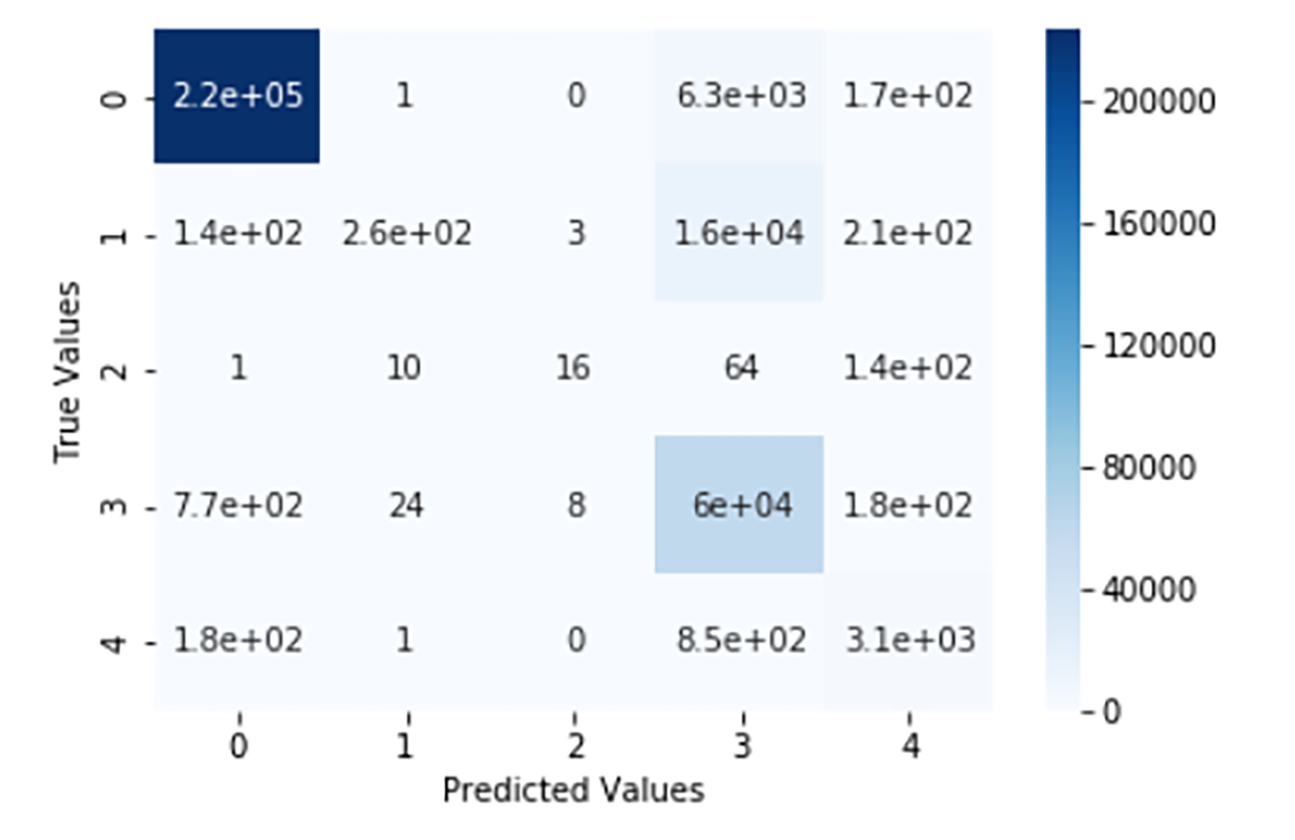
\includegraphics[width=1.0\columnwidth]{images/knnall.PNG}
	\caption{KNN Confusion Matrix - Multi-class classification}
	\label{F:knnall}
\end{figure}
Figure \ref{F:knnall} shows the multi-class confusion matrix for KNN.\\
The overall accuracy, recall, precision and F1 score for the 2-class classification are as follows: 92.35, 94.64, 85.95 and 89.20 percent. The same for the multi-class classification are as follows: 92.08, 55.90, 80.16
and 55.17. We can observe that the accuracy of the model increases as compared to a simple logistic regression model for the 2-class classification. The recall and F1 scores too increase for the multi-class classification case.

\subsubsection{Support Vector Machine - Linear}
A Support Vector Machine is a model based on the maximal margin classifier i.e. classification based on an optimal separating hyperplane. The support vector machine extends this concept further and to non-linear decision boundaries as well (cite9).\\
We train two linear SVM models - one for the 2-class classification and one for the multi-class classification. 
\begin{figure}
	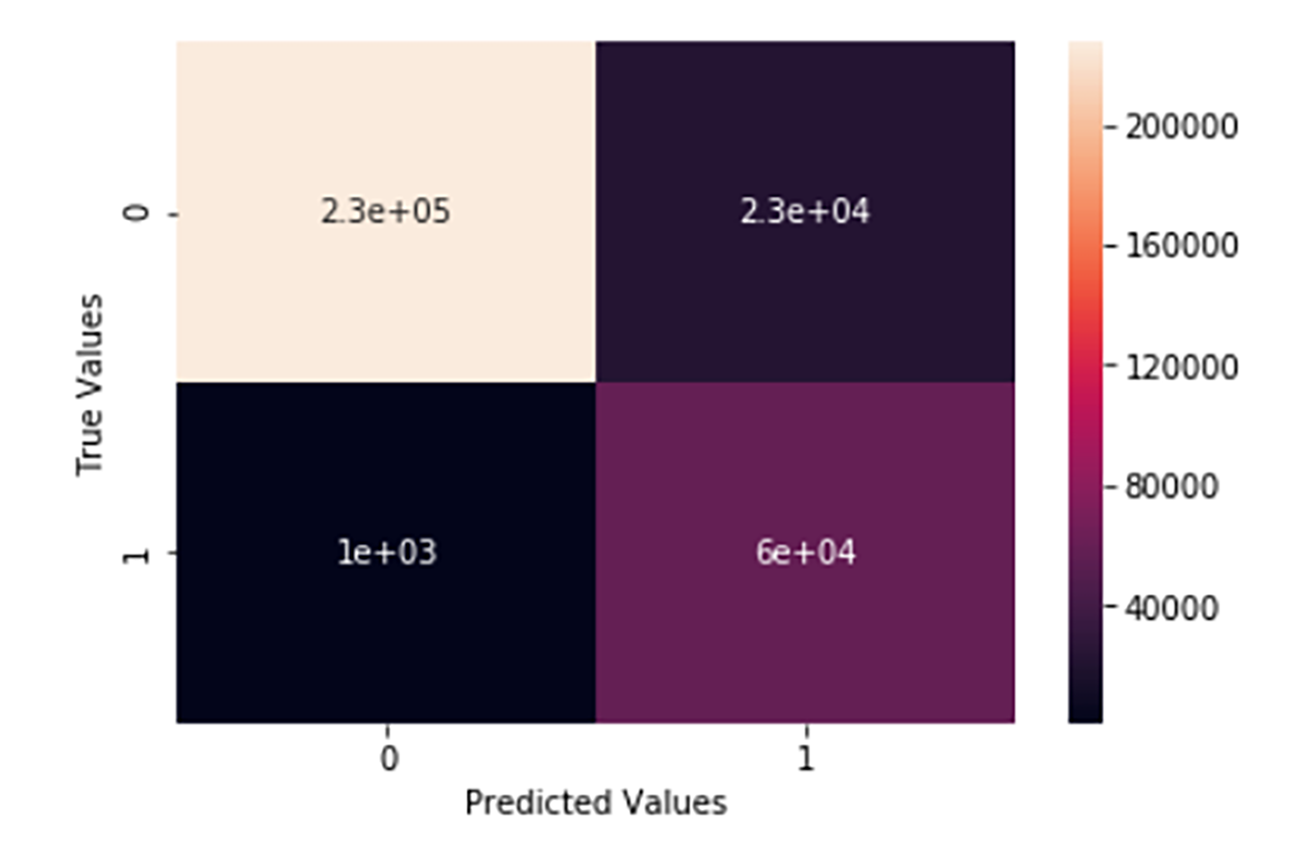
\includegraphics[width=1.0\columnwidth]{images/svm2.PNG}
	\caption{Linear SVM Confusion Matrix - 2-class classification}
	\label{F:linsvm2}
\end{figure}
Figure \ref{F:linsvm2} shows the 2-class confusion matrix for linear SVM.
\begin{figure}
	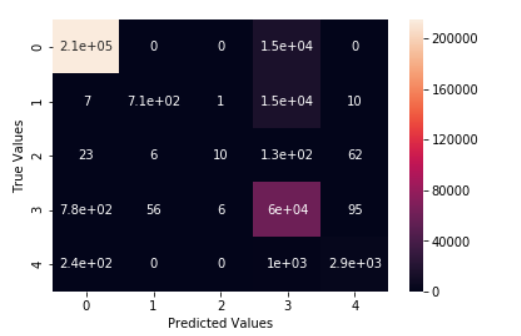
\includegraphics[width=1.0\columnwidth]{images/svmall.PNG}
	\caption{Linear SVM Confusion Matrix - Multi-class classification}
	\label{F:linsvmall}
\end{figure}
Figure \ref{F:linsvmall} shows the multi-class confusion matrix for linear SVM.\\
The overall accuracy, recall, precision and F1 score for the 2-class classification are as follows: 92.24, 94.55, 85.80 and 89.06 percent. The same for the multi-class classification are as follows: 89.29, 53.96, 81.97 and 54.22. We can observe that the accuracy of the model increases as compared to a simple logistic regression model but is lower than the KNN model for the 2-class classification. The recall and F1 scores too increase compared to logistic regression but are lower than KNN for the multi-class classification case.

\subsubsection{Support Vector Machine - Polynomial}
Here, we train two SVM models (with polynomial kernels of degree=3) - one for the 2-class classification and one for the multi-class classification. 
\begin{figure}
	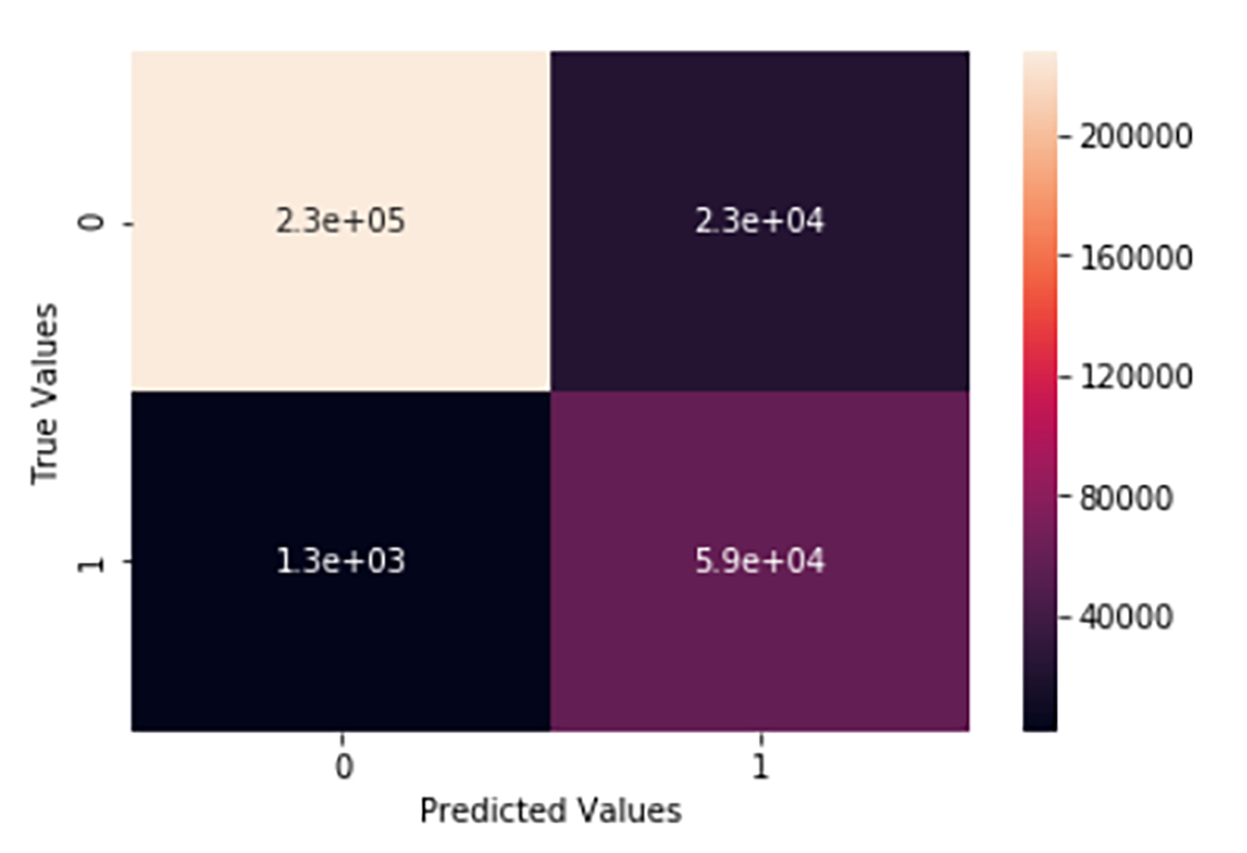
\includegraphics[width=1.0\columnwidth]{images/svmpoly2.PNG}
	\caption{Polynomial SVM Confusion Matrix - 2-class classification}
	\label{F:polysvm2}
\end{figure}
Figure \ref{F:polysvm2} shows the 2-class confusion matrix for polynomial SVM.
\begin{figure}
	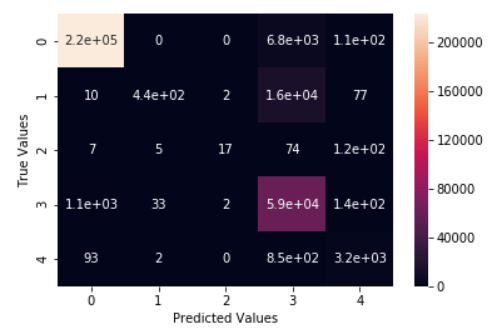
\includegraphics[width=1.0\columnwidth]{images/svmpolyall.PNG}
	\caption{Polynomial SVM Confusion Matrix - Multi-class classification}
	\label{F:polysvmall}
\end{figure}
Figure \ref{F:polysvmall} shows the multi-class confusion matrix for polynomial SVM.\\
The overall accuracy, recall, precision and F1 score for the 2-class classification are as follows: 92.26, 94.39, 85.84 and 89.05 percent. The same for the multi-class classification are as follows: 91.96, 56.49, 86.28
and 56.42. We can observe that the accuracy of this model too is lower than the KNN model for the 2-class classification. However, the recall and F1 scores are higher than KNN too (correctly classifies more DoS/DDoS and probe attacks than linear SVM and more R2L and probe attacks than KNN) for the multi-class classification case. Overall, the performance is similar to KNN.

\subsubsection{Random Forest}
A random forest model works as an improvement over individual decision trees through building a number of decision trees on bootstrapped samples along with decorrelating the individual trees by choosing only a random subset of predictors out of the total predictors while constructing trees. At each split, a fresh subset of predictors is used (cite9).\\
We train two random forest models - one for the 2-class classification and one for the multi-class classification. 
\begin{figure}
	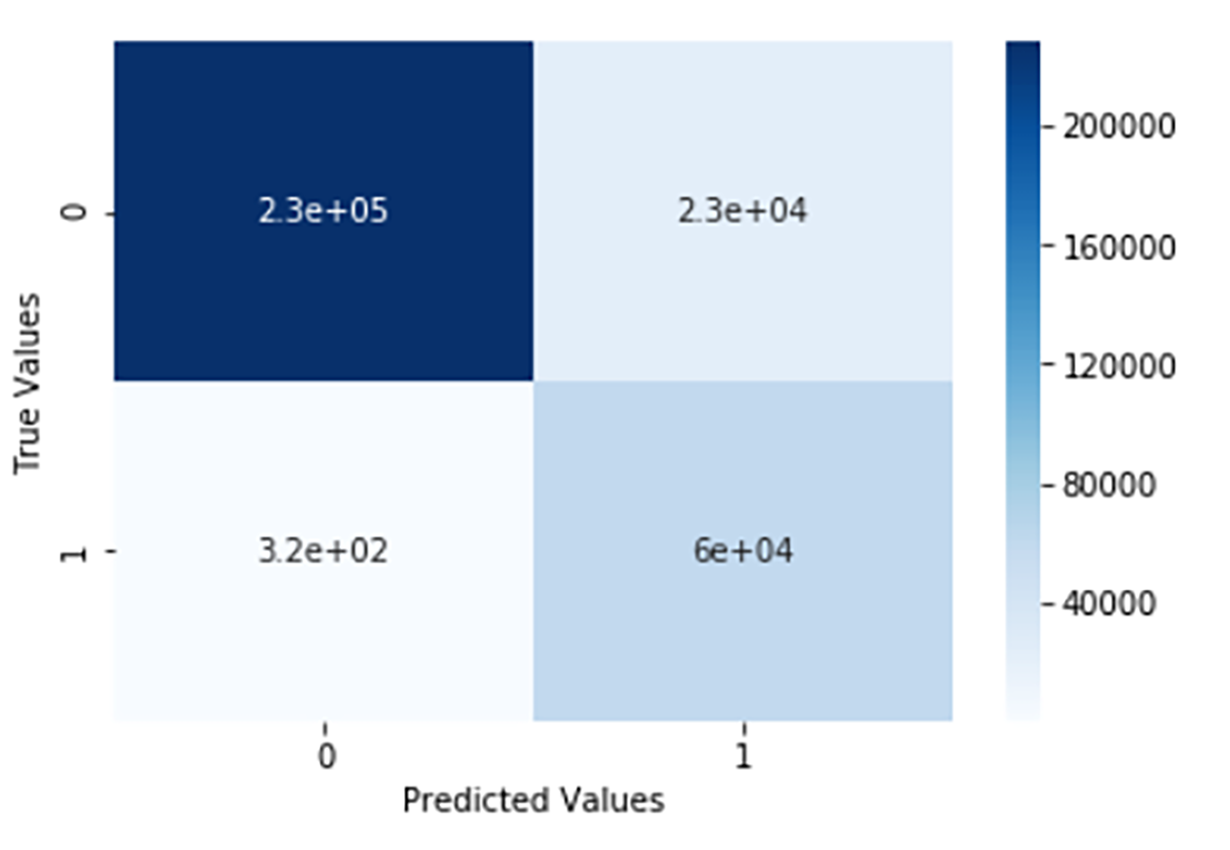
\includegraphics[width=1.0\columnwidth]{images/rf2.PNG}
	\caption{Random Forest Confusion Matrix - 2-class classification}
	\label{F:rf2}
\end{figure}
Figure \ref{F:rf2} shows the 2-class confusion matrix for a Random Forest.
\begin{figure}
	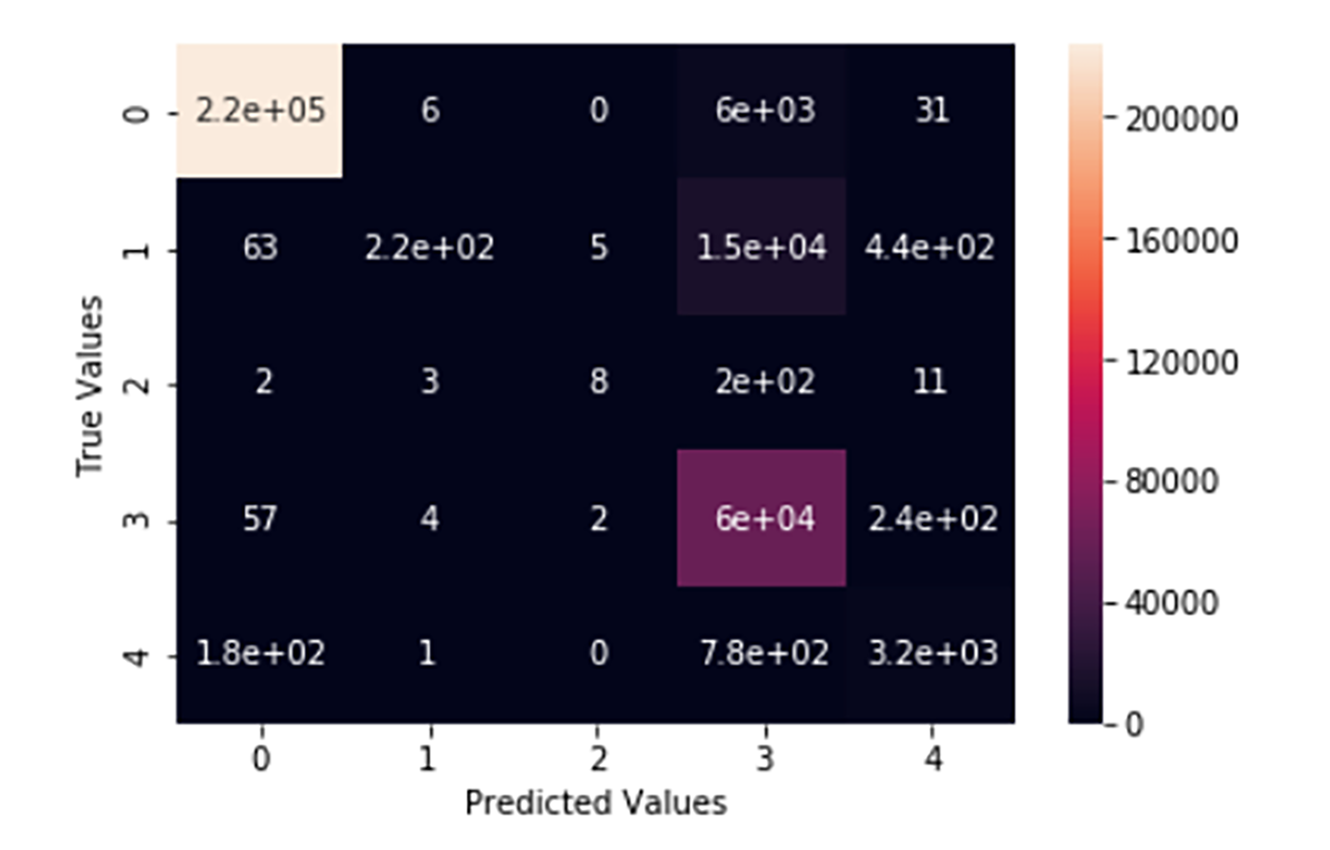
\includegraphics[width=1.0\columnwidth]{images/rfall.PNG}
	\caption{Random Forest Confusion Matrix - Multi-class classification}
	\label{F:rfall}
\end{figure}
Figure \ref{F:rfall} shows the multi-class confusion matrix for a Random Forest.\\
The overall accuracy, recall, precision and F1 score for the 2-class classification are as follows: 92.64, 95.22, 86.31, 89.63 percent. The same for the multi-class classification are as follows: 92.44, 55.74, 80.39
and 54.26. We can observe that the accuracy of this model higher than all the previous models for the 2-class classification. The recall and F1 score for multi-class classification is comparable to the SVM models.

\subsubsection{Neural Networks : Multi-Layer Perceptron}
Neural Networks are soft-computing techniques that attempt to replicate information processing in biological systems, and thus have excellent learning capabilities. When used for pattern recognition or classification purposes, the most useful Neural Network is that of Multi-Layer Perceptron which basically acts as multiple layers of logistic regression models (cite10).\\
We train two MLP models (with a hyperbolic tan activation function as it has better convergence properties than a logistic or sigmoid function) - one for the 2-class classification and one for the multi-class classification. 
\begin{figure}
	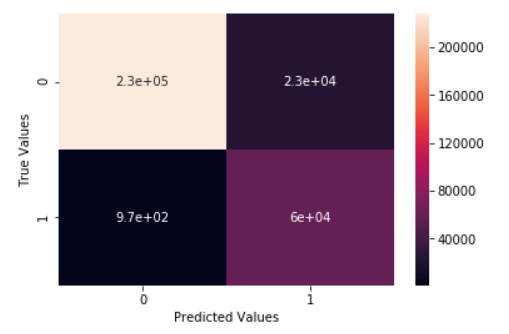
\includegraphics[width=1.0\columnwidth]{images/nn2.PNG}
	\caption{Multi-Layer Perceptron Confusion Matrix - 2-class classification}
	\label{F:nn2}
\end{figure}
Figure \ref{F:rf2} shows the 2-class confusion matrix for a Multi-Layer Perceptron.
\begin{figure}
	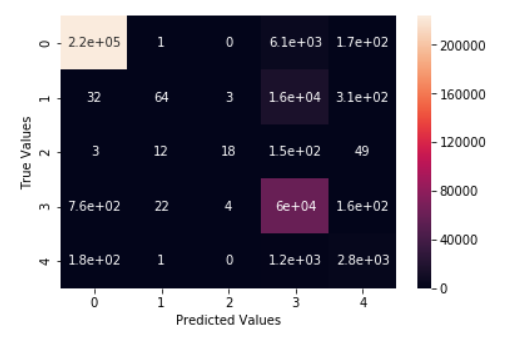
\includegraphics[width=1.0\columnwidth]{images/nnall.PNG}
	\caption{Multi-Layer Perceptron Confusion Matrix - Multi-class classification}
	\label{F:nnall}
\end{figure}
Figure \ref{F:nnall} shows the multi-class confusion matrix for a Multi-Layer Perceptron.\\
The overall accuracy, recall, precision and F1 score for the 2-class classification are as follows: 92.40, 94.68, 86.02 and 89.27 percent. The same for the multi-class classification are as follows: 91.98, 54.18, 77.53
and 53.90. We can observe that the accuracy of this model is similar to that of a random forest model for the 2-class classification. The recall and F1 score for multi-class classification is comparable to the random forest and linear SVM model.

\subsubsection{Ensemble Modeling}
Ensemble modeling deals with the combination of two or more machine learning models to generate a model with better accuracy. We have already observed that Random Forests have the highest accuracy for the 2-label classification whereas a polynomial SVM has better recall for the multi-label classification. Therefore, we try to get the best of both worlds by creating an ensemble of two Random Forest (with different rules for selection of the feature subset) and one polynomial SVM model.\\
We train two ensemble models - one for the 2-class classification and one for the multi-class classification. 
\begin{figure}
	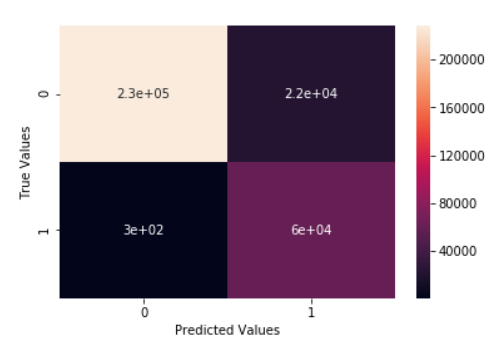
\includegraphics[width=1.0\columnwidth]{images/ensemble2.PNG}
	\caption{Ensemble Model Confusion Matrix - 2-class classification}
	\label{F:en2}
\end{figure}
Figure \ref{F:en2} shows the 2-class confusion matrix for an ensemble model.
\begin{figure}
	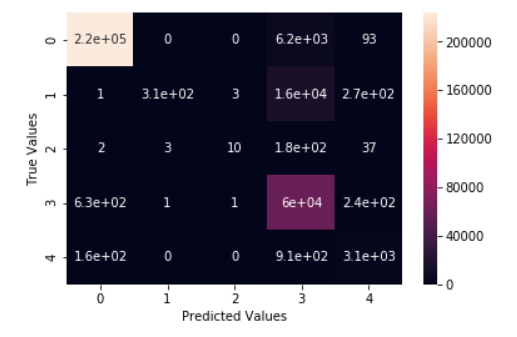
\includegraphics[width=1.0\columnwidth]{images/ensembleall.PNG}
	\caption{Ensemble Model Confusion Matrix - Multi-class classification}
	\label{F:enall}
\end{figure}
Figure \ref{F:enall} shows the multi-class confusion matrix for an ensemble model.\\
The overall accuracy, recall, precision and F1 score for the 2-class classification are as follows: 92.69, 95.27, 86.37 and 89.69 percent. The same for the multi-class classification are as follows: 92.16, 55.31, 85.00
and 54.46. We can observe that the accuracy and F1 score of this model is  higher than all individual models for the 2-class classification. The recall and F1 score for multi-class classification is balanced between that of the random forest and the polynomial SVM but is higher than most individual models.

\subsubsection{Unsupervised Learning - Clustering}
Up till here, we observed and evaluated a variety of supervised learning models. As a result, we came to the conclusion that an ensemble of two good models often results in a better and more balanced result than individual models. In this section, we will examine how exploring the test data by means of a clustering algorithm (with no support from the training data) helps provide a good idea of the patterns within the data.\\
We train two k-means clustering models for both 2-class and multi-class classification - one for clusters=5 and the other for clusters=10 (for greater granularity). \\
\begin{figure}
	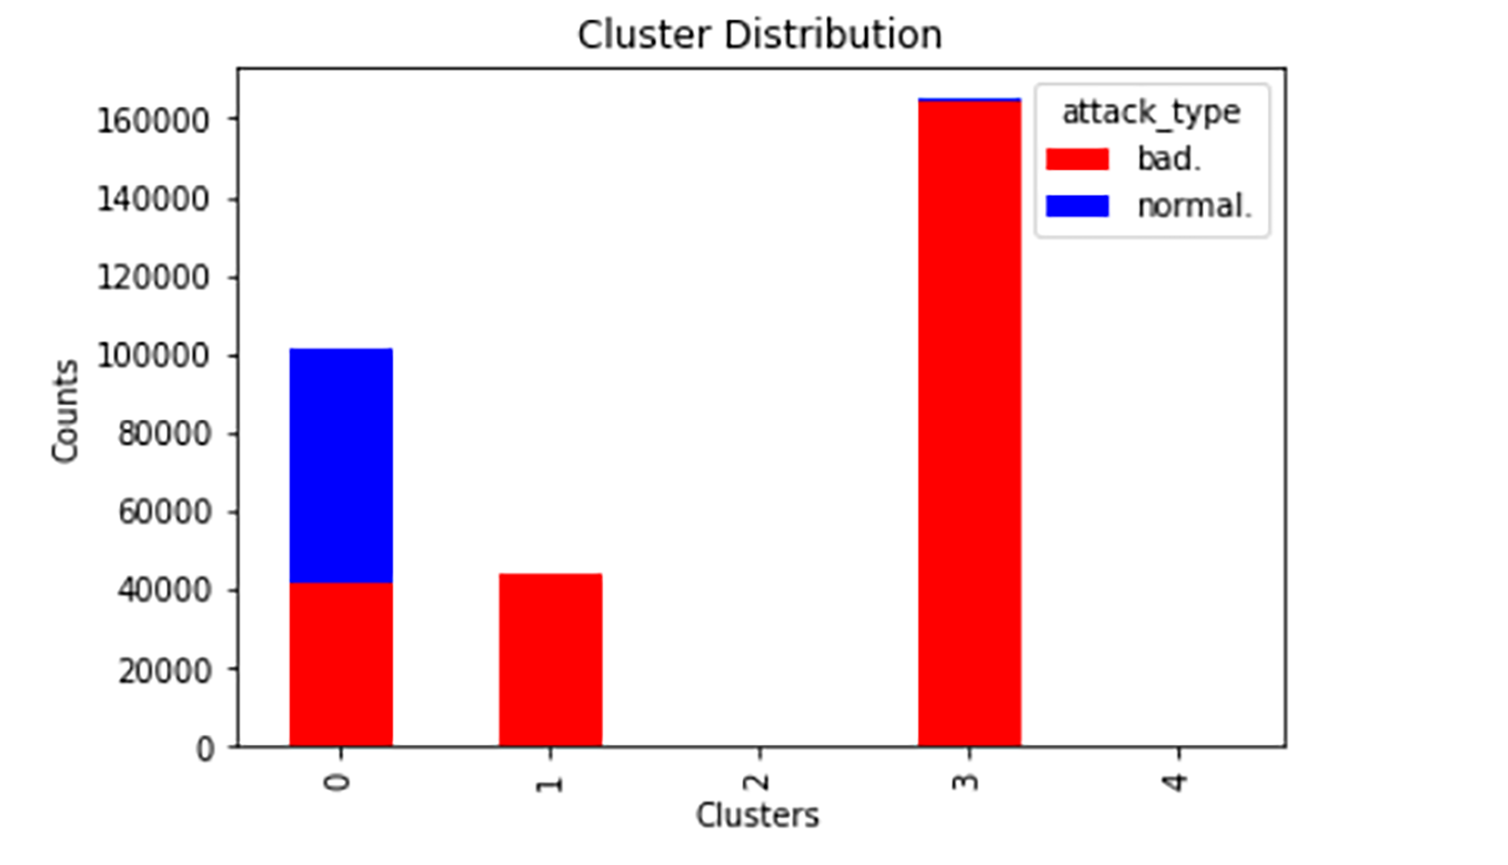
\includegraphics[width=1.0\columnwidth]{images/cluster52graph.PNG}
	\caption{Chart for k-means clustering (clusters=5) - 2-class classification}
	\label{F:cg52}
\end{figure}
Figure \ref{F:cg52} shows the 2-class chart for k-means clustering with clusters=5 (some clusters not visible due to small size).\\
We see that most of the clusters show one of the classes as a dominant proportion of the cluster. We can validate the same by comparing with the multi-class labels as well.\\
\begin{figure}
	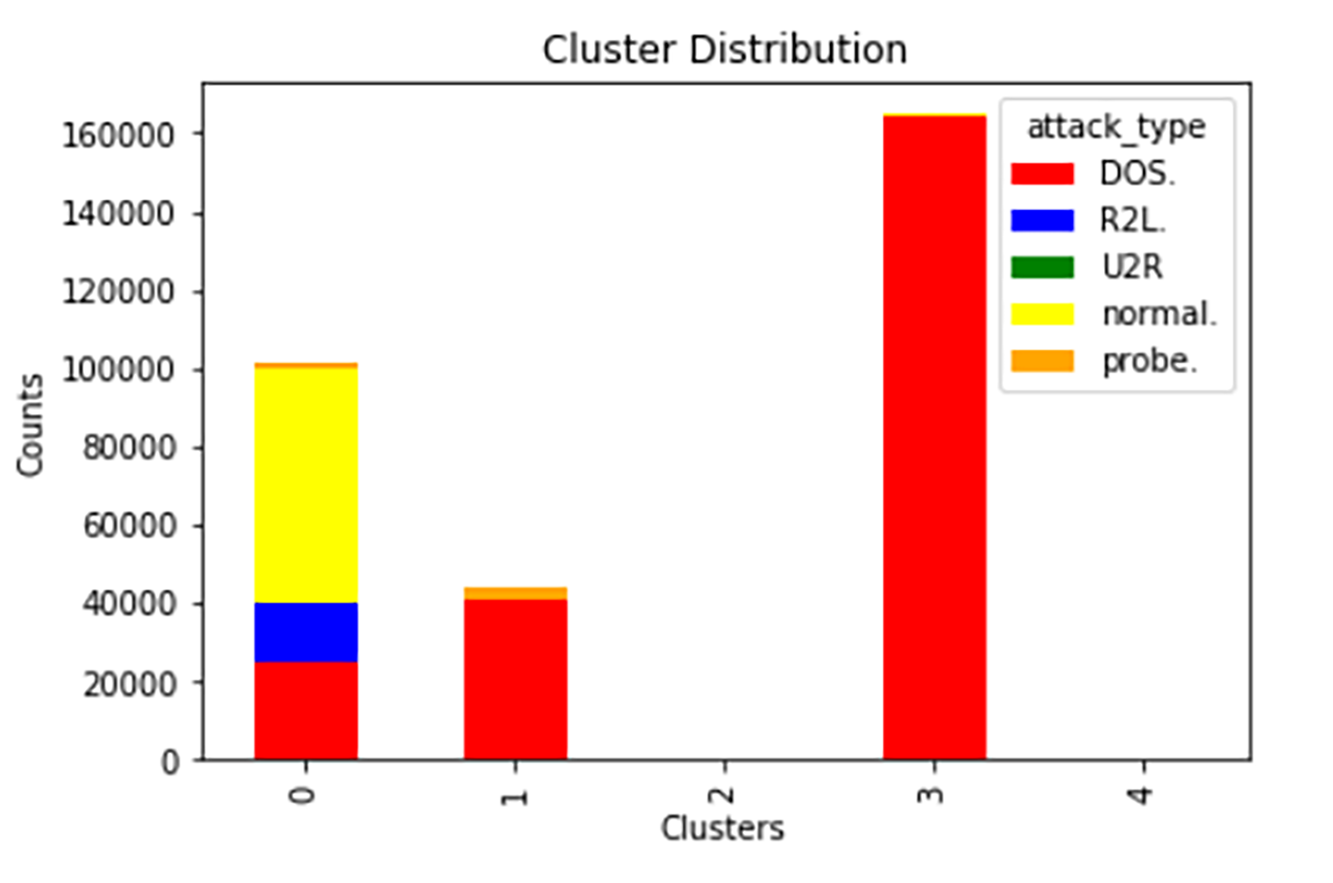
\includegraphics[width=1.0\columnwidth]{images/cluster5allgraph.PNG}
	\caption{Chart for k-means clustering (clusters=5) - multi-class classification}
	\label{F:cg5all}
\end{figure}
Figure \ref{F:cg5all} shows the multi-class chart for k-means clustering with clusters=5 (some clusters not visible due to small size).\\
We also run the analysis for clusters=10, for greater granularity.
\begin{figure}
	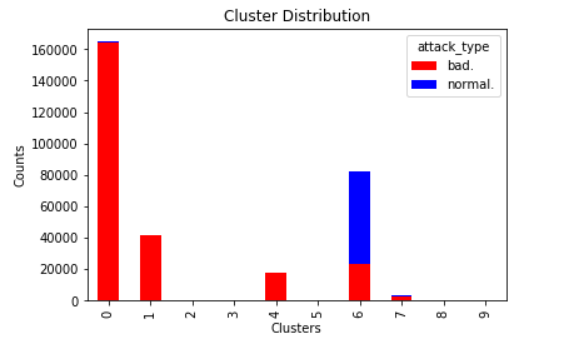
\includegraphics[width=1.0\columnwidth]{images/cluster102graph.PNG}
	\caption{Chart for k-means clustering (clusters=10) - 2-class classification}
	\label{F:cg102}
\end{figure}
Figure \ref{F:cg102} shows the 2-class chart for k-means clustering with clusters=10 (some clusters not visible due to small size).\\
\begin{figure}
	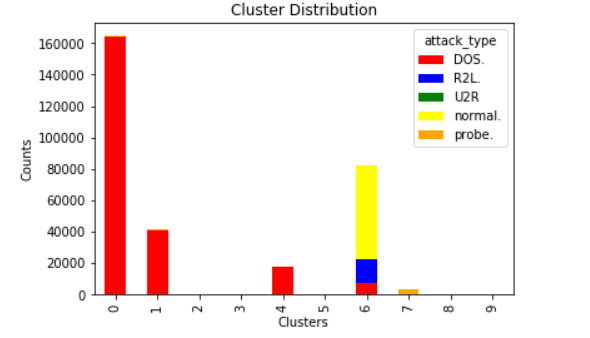
\includegraphics[width=1.0\columnwidth]{images/cluster10allgraph.PNG}
	\caption{Chart for k-means clustering (clusters=10) - multi-class classification}
	\label{F:cg10all}
\end{figure}
Figure \ref{F:cg10all} shows the multi-class chart for k-means clustering with clusters=10 (some clusters not visible due to small size).\\
We can observe the same trend here as well.

\subsection{Results}
Among the supervised models, we observe that on comparison, some models perform better in terms of accuracy whereas some perform better in terms of recall. We also observe that most models find it easier to perform a 2-class classification (due to the high volume of attack labels in both the datasets as compared to normal labels), but face difficulties in identifying the individual classes (especially R2L and U2R which have a higher proportion in the test data compared to the training data). Overall, for the purpose of DoS/DDoS and intrusion detection, we see that most machine learning models give good results (KNN for example), and an ensemble of a random forest and polynomial SVM model gives the best accuracy among all.\\
When we venture into unsupervised learning we observe that clustering algorithms too can work well on network traffic data by creating clusters of traffic logs through pattern recognition. Though clustering does not provide us with exact labels, it can be useful in cases where we do not have any training or benchmark data, by giving us a fair idea of the direction in which to proceed.

\section{Apache Spark - Using PySpark}
The volume of network traffic data generated is generally quite huge, and thus requires Big Data technologies to deal with it. Our demonstration was for a smaller subset of the actual dataset (which in itself consists of five million records). However, this larger dataset too consists of logs only for seven weeks of monitoring. We can therefore imagine how voluminous the datasets would begin to get with constant monitoring of systems. In such cases, Big Data cloud technologies can come to the aid of analytics, and help create a sustainable system for such intrusion detection purposes.\\
Our analysis was carried out using Python on an individual system. But often for larger datasets, we need additional resources. The PySpark API, from Apache Spark (an open-source processing engine), can help us  gain ``access to the extremely high-performance data processing enabled by Spark's Scala architecture - without the need to learn any Scala'' (cite11). The smallest building blocks of Spark are referred to as RDDs (Resilient Distributed Datasets) and these along with Spark's DataFrame can act as useful alternatives to the {\em Pandas} data frames, in case of large datasets, where the distributed processing power of Spark can come into play (cite11).\\
We can install PySpark on a Windows machine using GOW (incorporates Linux commands in Windows like gzip, curl and tar) and Anaconda (an open-scale distribution containing Jupyter Notebook and other resources for Python) (cite12). The package can be installed from the Apache Spark website, following which we perform {\em gzip} and {\em tar} operations on it. After adding the windows binary for Hadoop and modifying a few environment variables, you can launch Spark locally from Command Prompt. 
\begin{figure}
	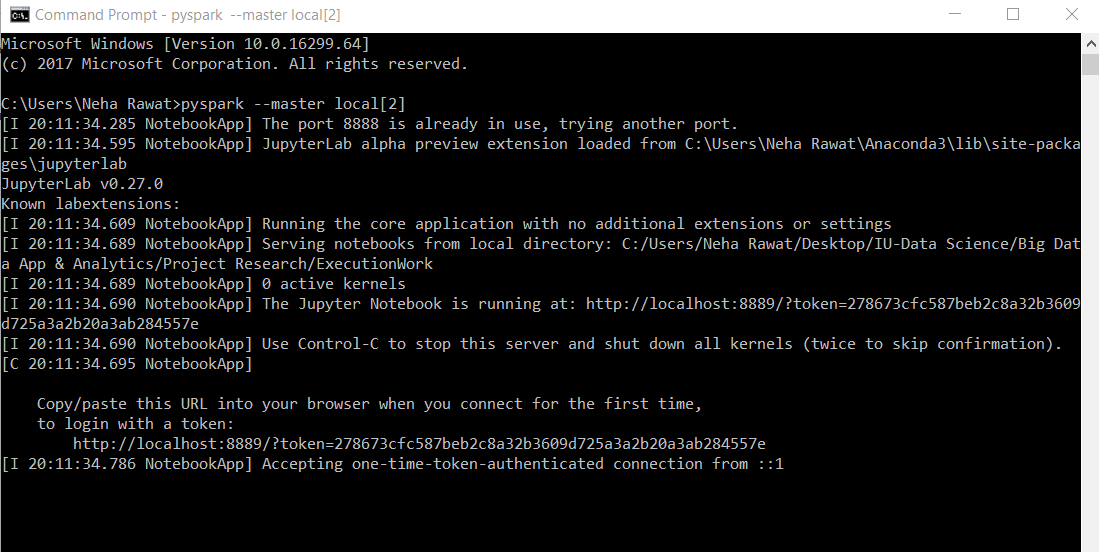
\includegraphics[width=1.0\columnwidth]{images/pyspark.PNG}
	\caption{Launching PySpark}
	\label{F:ps}
\end{figure}
Figure \ref{F:ps} shows the command prompt when we launch PySpark locally.\\
We have not used Spark for our analyses further as Python was able to handle the 10 percent datasets locally. However, PySpark can prove to be a great tool for analyzing data and creating models for larger datasets using a familiar and flexible language like Python.

\section{Conclusion}
The detection and prevention of DDoS attacks is a crucial problem for the safety and stability of networks. With the increasing use and dependence on technology and connectivity, this affects a huge cohort of people today. The data generated from day-to-day network traffic is huge and largely unstructured, but it can be captured and modified into an understandable structure, to be analyzed and used to generate efficient solutions. Through our analysis, we affirm the efficiency of machine learning technologies as tools for Big Data analytics and the use of open-source distributed processing systems as supports towards utilization of these tools. Therefore, Big Data technologies along with intelligent analytic solutions can help create new and improve existing defense systems to ensure security from such malicious attacks and intrusions. 

\bibliographystyle{ACM-Reference-Format}
\bibliography{report}